\documentclass{scrartcl}

\usepackage{graphicx}
\usepackage[siunitx, RPvoltages, european]{circuitikz}

\usepackage[ngerman]{babel}
\usepackage[utf8]{inputenc}
\usepackage{amsmath}
\usepackage{amssymb}
\usepackage[T1]{fontenc}
\usepackage{xcolor}
\usepackage{tikz}
\usepackage[breaklinks=true]{hyperref}
\usepackage[utf8]{inputenc}
\usepackage[babel,german=quotes]{csquotes}
\usepackage[style=numeric, backend=biber]{biblatex}
\usepackage{listings}
\usepackage{bytefield}
\usepackage{longtable}
\usepackage{sidecap}
\usepackage{wrapfig}

\addbibresource{ref.bib}

\graphicspath{ {../../images/} }

\KOMAoptions{parskip=full}


\begin{document}

    \title{Platinencomputer - Architektur}
    \author{Alexander Wersching und Simon Walter}
    \date{2022}
    \maketitle

    \newpage
    \tableofcontents

    \section{Idee}


    Vor ca. 2 Jahren hatte Alex die Idee, er wolle einen 8-bit Computer bauen, die vor 2 Jahren beim Regionalwettbewerb München-West eingereichte Version einer anderen Gruppe hat dann auch das Interresse von mir (Simon) geweckt.
    Ein paar monate später haben wir uns dann dazu entschieden, tatsächlich einen eigenen 8-bit-Computer zu bauen und haben auch bald angefangen erste Versuche auf dem breadboard zu machen.
    Es gab noch weder eine Möglichkeit diese erste Version automatisch zu betreiben, noch Daten zu schreiben/speichern, oder irgendwie mit der Umgebung zu interagieren, nur 3 Register 2 operationen und viele knöpfe zum Bedienen. [Bilder von v1].

    \newpage

    \section{Nützung von Platinen}
    \subsection{weshalb Platinen}

    \begin{wrapfigure}{r}{0.4\textwidth}
        \vspace{-40pt}
        \begin{center}
        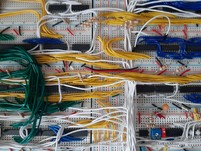
\includegraphics[width=0.37\textwidth]{Computer_V01_Chaos_07}
        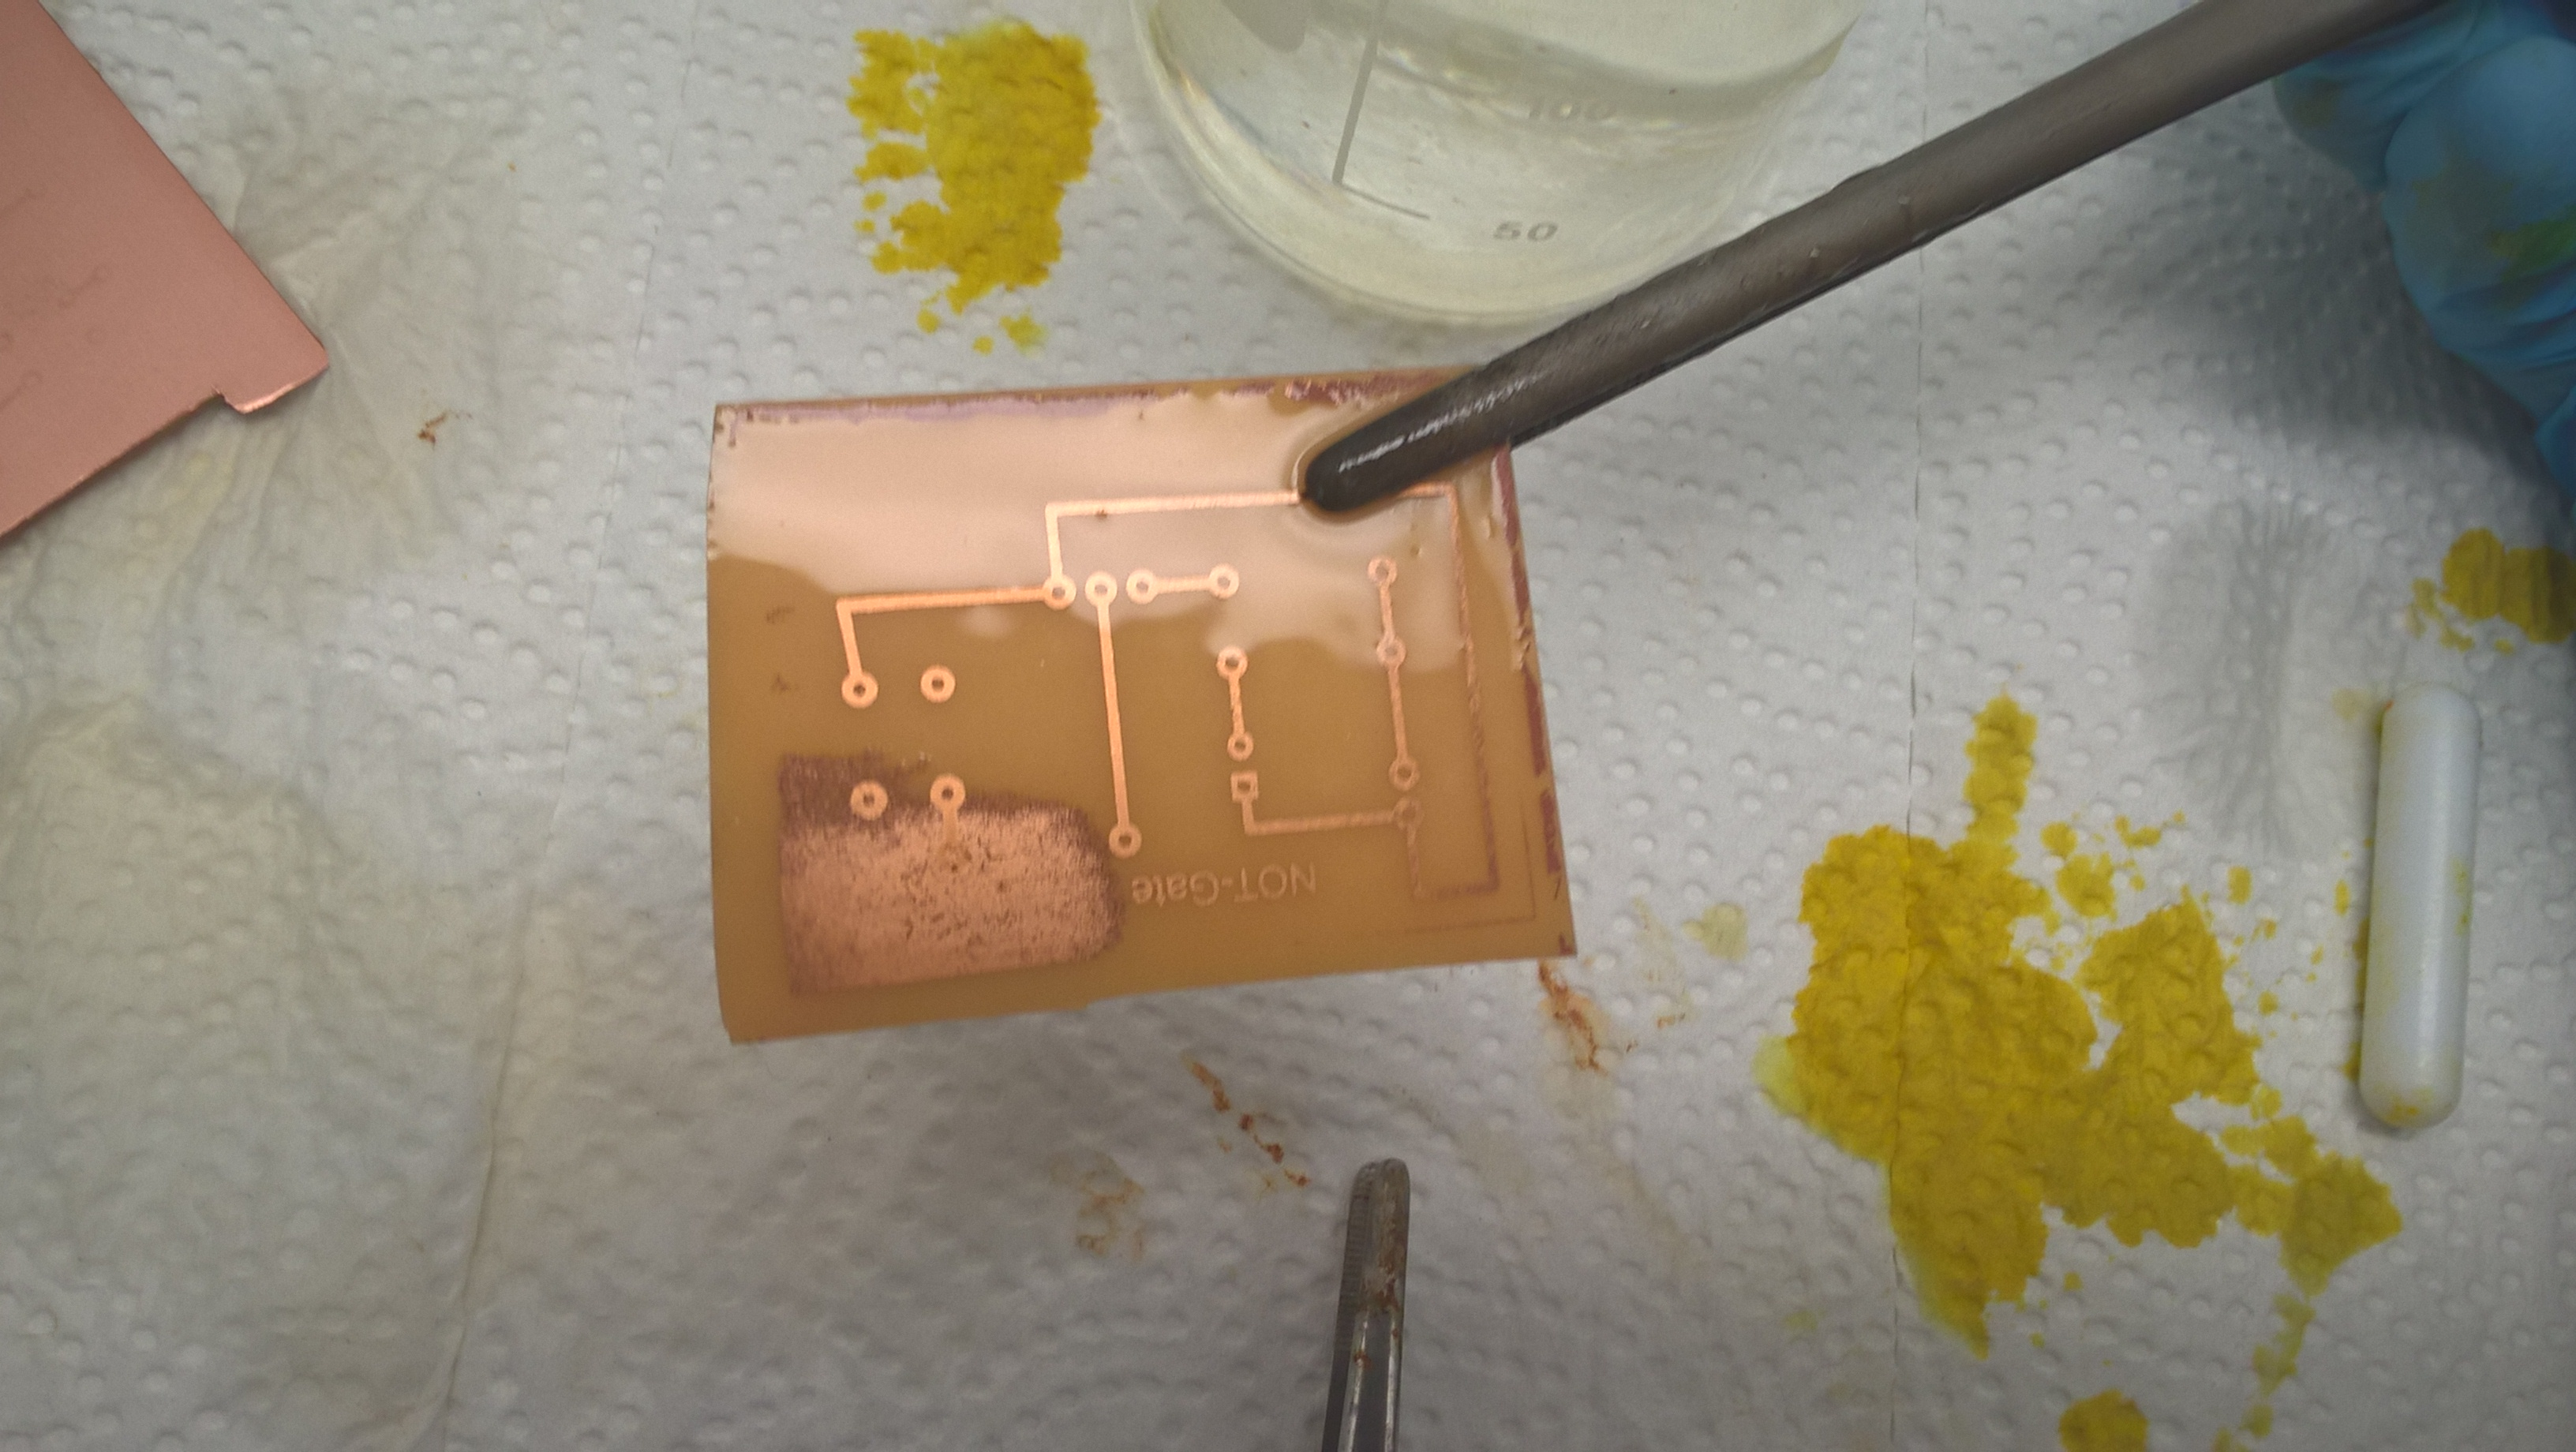
\includegraphics[width=0.37\textwidth,angle=0]{Handy/WP_20210704_20_54_21_Pro}
        \end{center}
        \vspace{-30pt}
    \end{wrapfigure}

    Bald war aber klar, dass ein einfaches Verwenden von flachen Kabel als Verbindung zwischen den Breadboards das Kabelgewirr, das wir bei dem Projekt von vor 2 Jahren gesehen haben
    und nach möglichkeit vermeiden wollten, um ein übersichtlicheres Design zu erreichen, nicht lösen kann.

    Auf der Suche nach einer Alternative sind wir fast zwangsläufig auf Platinen gekommen, aber weil unser Computer ja nicht mehr wirklich selbst gemacht wäre, wenn wir diese professionell Ätzen lassen würden,
    wollten wir versuchen - zumindest einen teil - selbst zu Ätzen, auch wenn wir dadurch natürlich auf viele Neue probleme gestoßen sind...




    \subsection{erste Versuche der Umsetzung}

    \begin{wrapfigure}{l}{0.4\textwidth}
        \vspace{-25pt}
        \begin{center}
        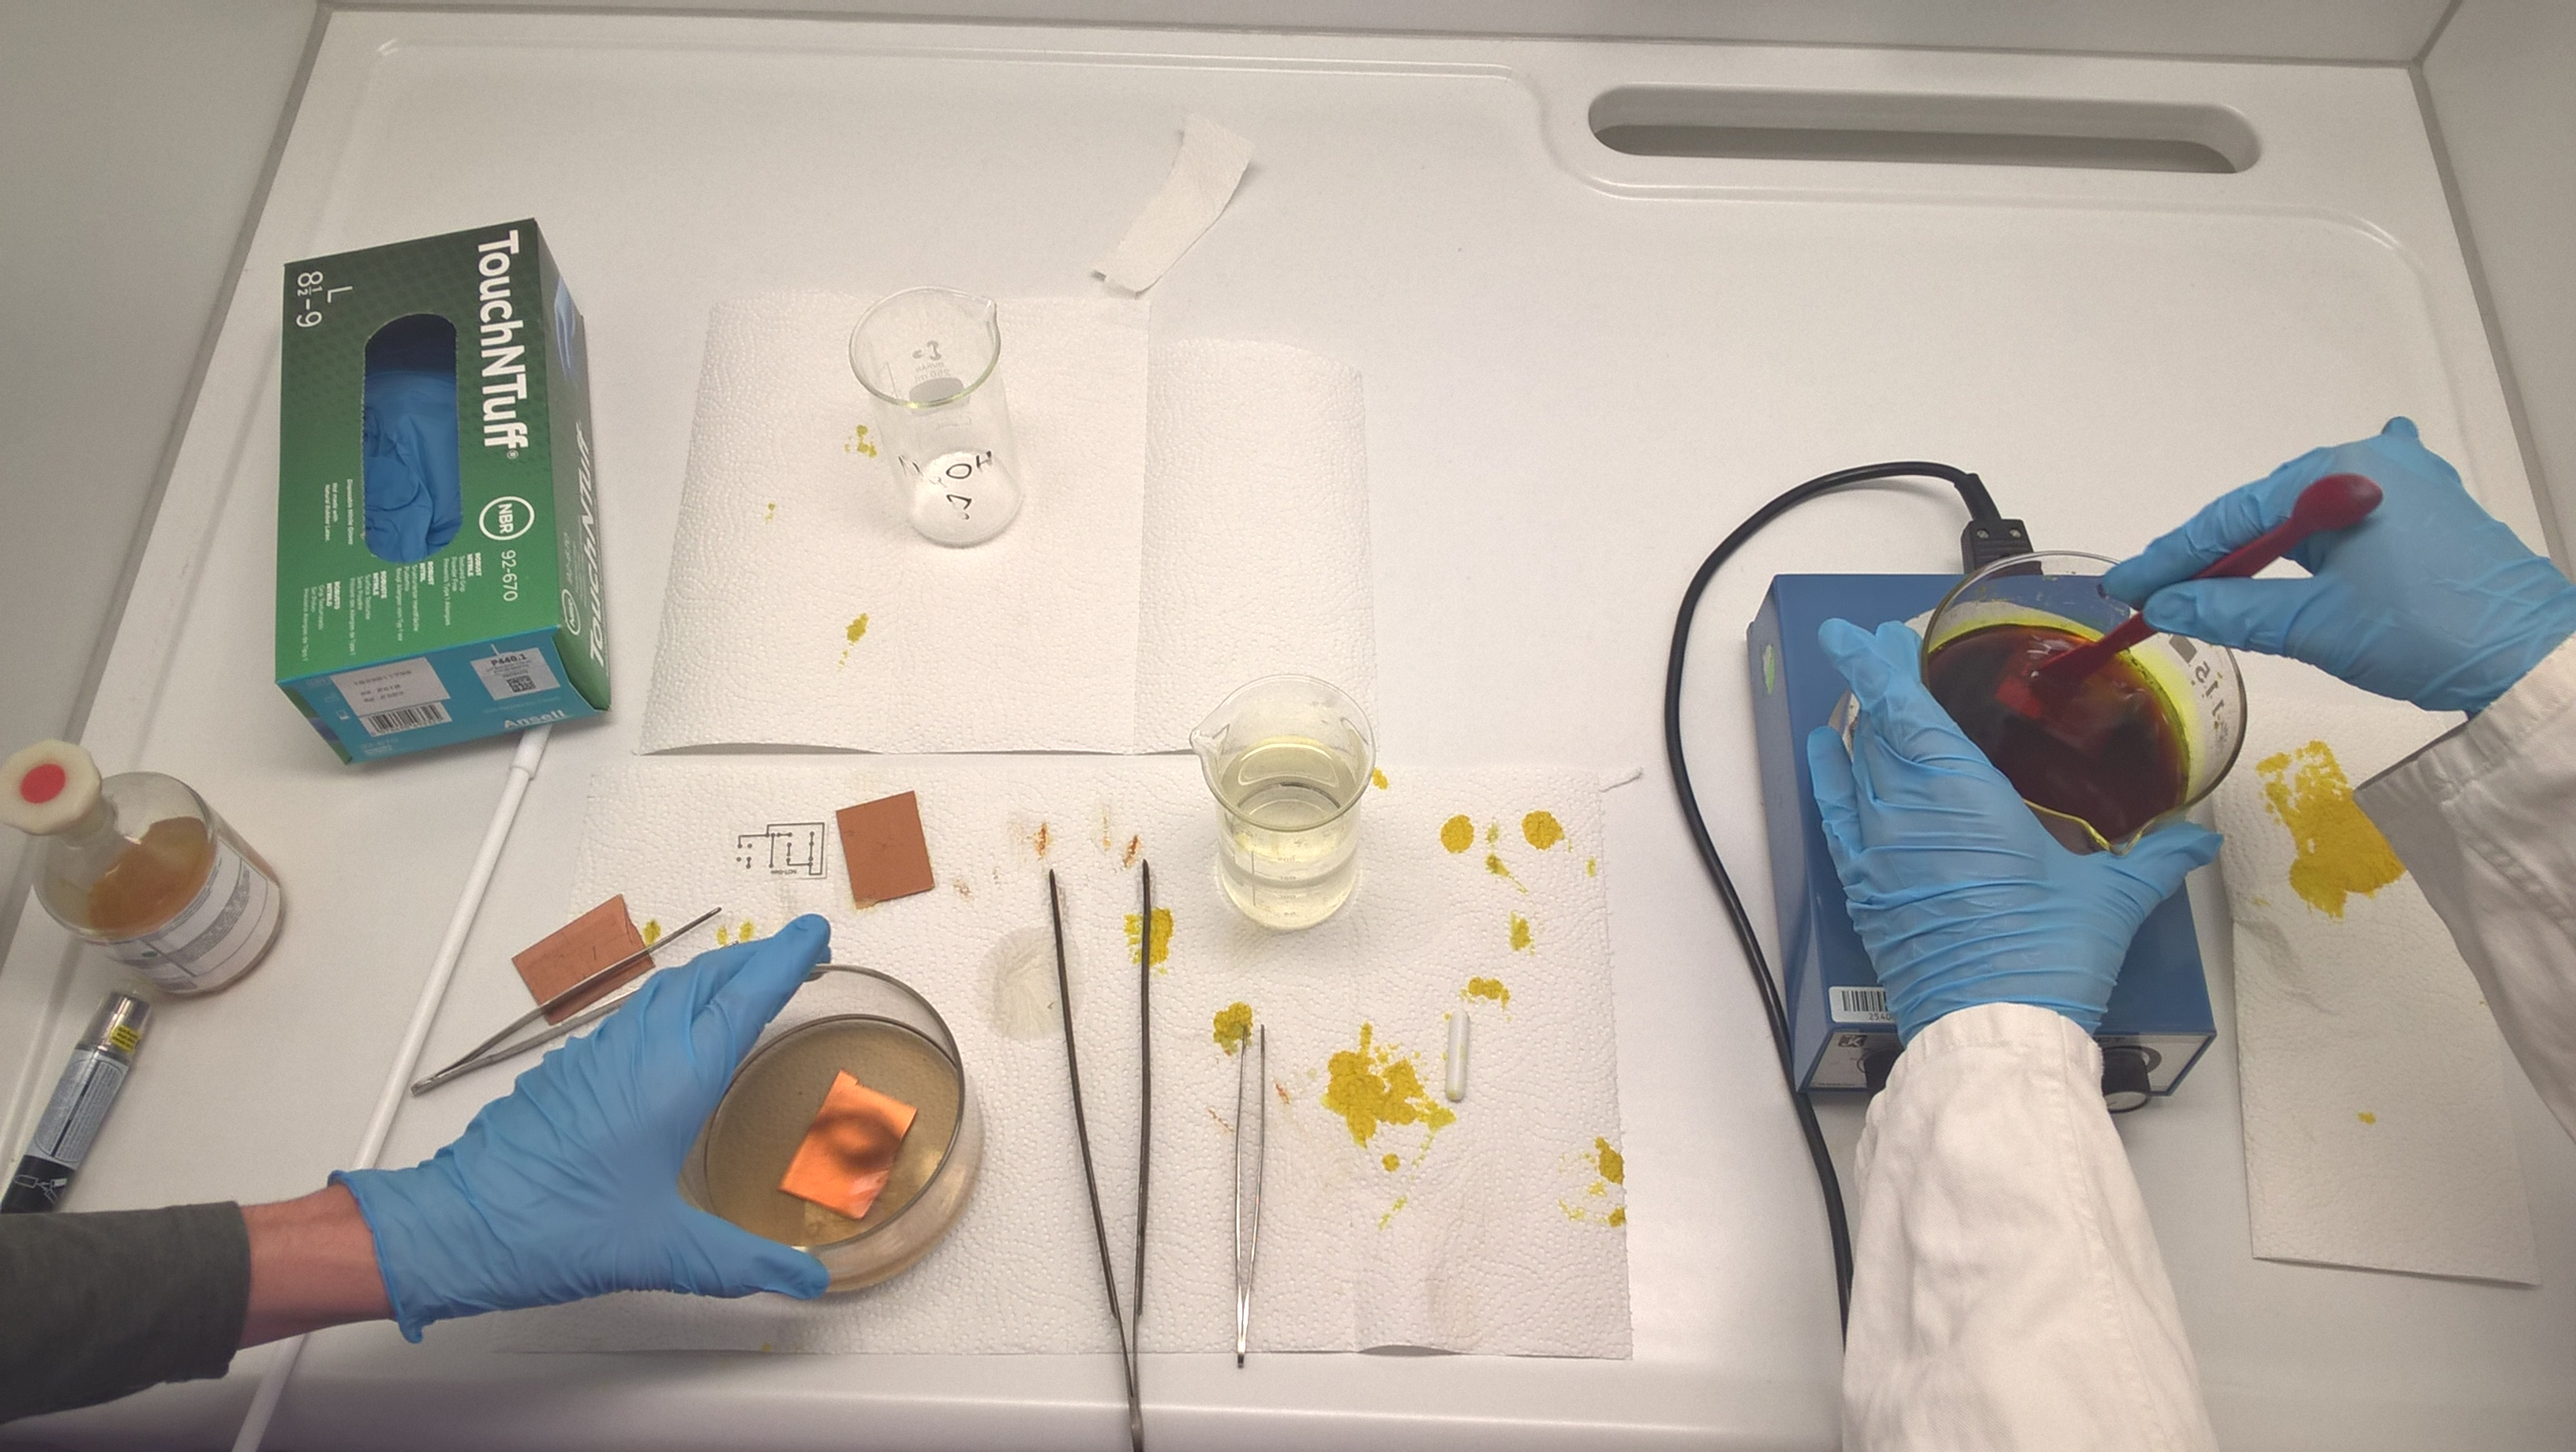
\includegraphics[width=0.4\textwidth,angle=0]{Handy/WP_20210704_20_40_03_Pro} %hier binn ich noch nicht ganz glücklich mit dem Bild
        \end{center}
        \vspace{-20pt}
    \end{wrapfigure}

    Was zu Beginn das Projekt vorangetrieben hat, ab diesem Punkt aber natürlich ein Problem dargestellt hat ist das Homeschooling, bei dem wir natürlich nicht Ätzen können.
    (wir hätten es natürlich zu Hause versuchen können, hatten da aber keine adequate Ausrüstung v.a. bzgl. Sicherheit)
    bis wir dann so weit waren erste Versuche zu machen war es dann schon Ende 2020.


    \subsection{design}

    %\begin{wrapfigure}{r}{0.5\textwidth}
    %    \vspace{-40pt}
    %    \begin{center}
    %    \end{center}
    %    \vspace{-30pt}
    %\end{wrapfigure}

    Nachdem es auch auf geätzten Platinen noch nicht automatisch ordentlich ist und eine Große Platine für uns nicht machbar gewesen wäre, haben wir uns dann noch ein 3-Dimensionales Design ausgedacht.

    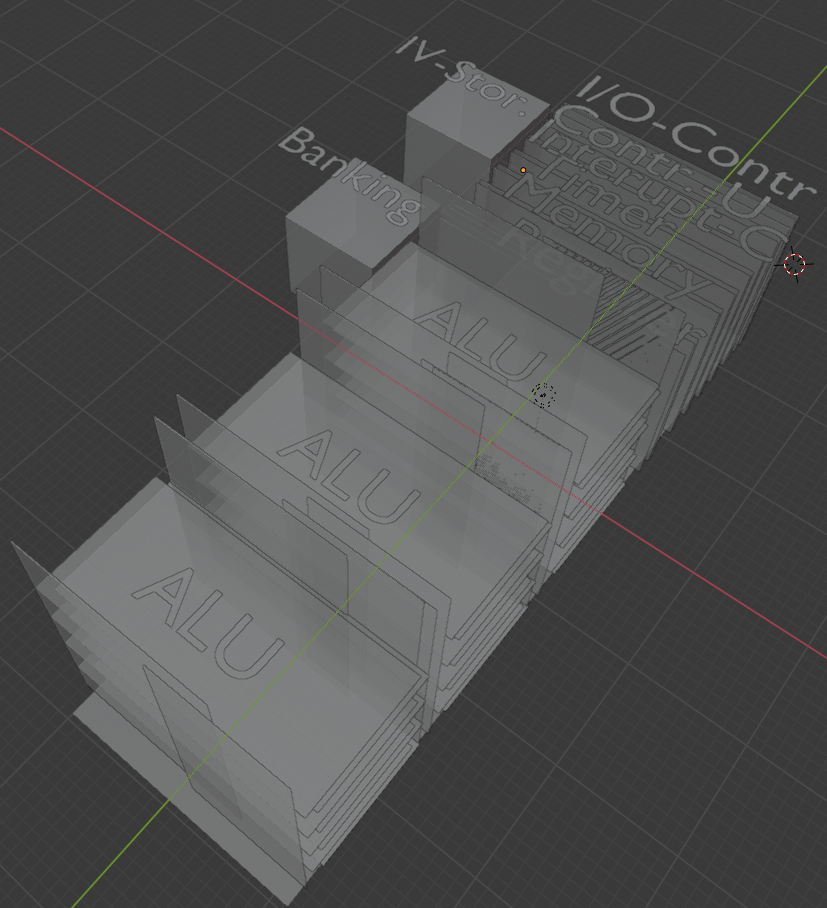
\includegraphics[width=0.5\textwidth]{3D_Desighn_V2}

    Offensichtlich ist das mit unseren aktuell geplanten Modulen: am Boden sitzt eine große Bus-Platine, auf der wie alle Module senkrecht aufstecken.

    \section{Anforderungen V1}
    Im nächsten Lockdown hatten wir dann wieder viel Zeit zu planen, und der geplante Computer wurde immer komplexer.
    \subsection{Datenlänge, Memory, Logik-Operationen und konditionale jumps}

    Aus 8-bit wurden 16-bit Datenlänge, wir wollten ein Memory-Modul haben, immer mehr Operationen bis hin zur Hardware-Multiplikation und komplexere konditionale Jumps.
    \subsection{IO-Ports}
    Dazu hat sich dann die Idee von einer komplexeren Umsetzung von Interaktion mit dem Computer eingeschlichen:
    universelle Ports zum Anschließen von (modifizierten) Festplatten, Sensoren, einfachen Tastaturen, LCD-Displays und der Vorstellung einer Grafikkarte, die echte Bildschirme betreiben kann.
    [spezifikation v0.1]

    \subsection{Berechtigungssysten}
    Die vermutlich die größte Änderung war danach, dass wir ein Berechtigungssystem einführen wollten.
    Dafür haben wir dann Flaggen, Interrupts und noch mehr Instruktionen hinzugefügt.
    \subsection{ROM}
    Um den Computer komplett unabhängig funktionsfähig machen zu können, haben wir uns dann überlegt einen Teil des RAMs durch ROM zu ersetzen, um automatisch Programme von einem externen Speichermedium laden zu können.
    \subsection{Banking}
    Nachdem uns $2^{16}$= 65536 Speicherzellen (jede einen 16-bit Wert beinhaltend) also 128kiB Daten in Memory bei so vielen Anforderungen dann doch etwas wenig erschienen
    und wir die Idee von mehreren Prozessen, die abwechselnd ausgeführt werden, verlockend war haben wir uns dann entschieden durch eine neue Instruktion, mit der wir Teile des Arbeitsspeichers auswechseln können (Banking),
    beides zu ermöglichen. [Link zu Dokumentation v0.2]

    \section{Tests}
    \subsection{Breadboard test}
    Zwischendurch haben wir dann für die Einladung zu einem lokalen Projekt $"Persvektive P"$ am 15.07.2021 wieder einen Prototyp auf dem Breadboard gebaut, wobei auch diese Version sehr unvollständig war.

    \subsection{Geschwindigkeit}
    Um einen eindruck zu bekommen, wie komplex unsere programme werden können, ohne übermäßig lange zu brauchen, haben wir dann versucht zu errechnen, wie schnell wir den Computer maximal laufen lassen können, ohne fehlerhafte Ergebnisse zu erhalten.
    Also haben den "Propagation-delay", die Zeit, bis der Chip den Output liefert, den der laut der Eingabe haben müsste, aller Komponenten gemessen, die wir verwenden wollen.
    die meisten Chips, die wir jetzt vorhaben zu verwenden haben eine Verzögerung von ungefähr 8 Nanosekunden, allerdings haben wir bei den verschiedenen versionen, die wir getestet haben, teilweise weitaus höhere Werte bis zu 150ns erreicht, was an sich noch nicht so schlecht ist, aber wenn wir damit rechnen, dass wir reihen von bis zu 40 Chips in einem Clock-Zyklus haben, limitiert das die Geschwindigkeit schon sehr.

    \subsection{Funktionsweise Chips}
    Wir wollen als basis für unseren Computer ja Chips kaufen, aber wie funktionieren die eigentlich?
    Wir haben also versucht den Aufbau herauszufinden, indem wir einfach einen geöffnet haben, wobei $"$Einfach$"$ nicht so ganz stimmt, weil die Hülle aus Epoxidharz besteht, was sich fast nicht auflösen lässt.
    Also mussten wir mechanisch abtragen, also Schleifen.

    \section{Umsetzung}
    \subsection{Programmierung}
    Um den ROM-Chip zu programmieren haben wir zwar mal kurz ein bisschen manuell über Schalter programmiert, aber nachdem das offensichtlich zu lange brauchen würde haben wir dann einen Arduino (um genau zu sein, einen ESP32) programmiert und an die pins des ROM-Ch8ips angeschlossen.
    Der Arduino bekommt die zu schreibenden bits wiederum aus einem Python-Programm, das den Assembler in Maschinensprache (1en und 0en) umwandelt.

    \subsection{weitere tests zum Ätzen}
    Im Schuljahr 2021-2022 haben wir dann wieder weitere Tests zum Ätzen - dieses mahl sowohl erfolgreicher, als auch besser Dokumentiert, um die optimalen Belichtungs- und Ätzzeiten zu finden.

    \subsection{Spezifikation}
    Gleichzeitig haben wir auch angefangen unsere erste vollständige Version der Spezifikation zu schreiben (jetzt auch mit dem eindeutigen Ziel es bei Jugend Forscht anzumelden, die vorherigen Versionen waren auf Englisch, weil wir es uns beim Programmieren der Einheitlichkeit halber angewöhnt haben alles in Englisch zu schreiben).

    \subsection{Desighnen der Schaltungen}

    \subsection{Ätzen der }
    Aktueller Bau: Ablauf...
    \subsection{Programme}
    Assembler/Emulator


\end{document}